\chapter{Theory}
\lhead{\emph{Theory}}

\section{Handwriting recognition}
% history
% on-line and off-line
% problems related, preprocessing, segmentation, classification of symbols, continuous input
% 
Since the ancient days of computers, handwriting recognition has been continuously researched \cite{simon_off-line_1992}. % dank source brah :D

The goal of a handwriting recognition system is to correctly classify text with as high accuracy as possible. To do this, the system will have to be able to segment the different symbols and classify each of them. How the system does this depends on the format of the input data.

[Image that illustrates the segmentation problem and classification problem, maybe 2]

There are mainly two approaches the input data, online and offline (kilde). Online recognition uses data from pen strokes such as sampled coordinates of pen movements and the time difference between them. On the other side, offline recognition uses only static data like images. A major difference between these approaches is that online recognition has access to a time dimension, the order of the pen strokes and coordinates is known. 
%This can in some ways aid in segmenting correctly. For example, pen strokes that overlap can be separated with access to the time dimension. 

[Image that illustrates online and offline HWR]



\subsection{Existing solutions}
% Scientific
% Commercial
% Methods they used
% 
% mathpix
% myscript
% microsoft word has
As handwriting recognition is a very well known problem, many have tried to solve it.

The methods used


\subsection{CROHME}


\subsection{InkML}
InkML is an markup language based on XML to describe digital ink data. The format is specified by the World Wide Web Consortium \cite{chee_ink_2011}. InkML groups it's content in specific XML-style elements called ink, the ink element often has sub elements which is a trace element.\\

\begin{minipage}{\linewidth}
\begin{lstlisting}[language=XML, %
label={lst:InkML_ex},
caption={Example of three traces, each with an file-unique id. In addition to traces, we have listed a tracegroup, which specifies what and where the traces belong to. Truths are used when providing labels to use in supervised learning, which is explained later in this chapter.}]
<trace id="0">
    207 136, 199 141, 197 143, 196 144, 195 146, 194 147, 193 149
</trace>
<trace id="1">
    847 201, 847 204, 846 207, 846 211, 846 215, 845 219, 845 222
</trace>
<trace id="2">
    833 235, 822 235, 821 235, 820 235, 819 236, 819 235, 819 236
</trace>

<traceGroup xml:id="3">
	<annotation type="truth">+</annotation>
	<traceView traceDataRef="1"/>
	<traceView traceDataRef="2"/>
	<annotationXML href="+_1"/>
</traceGroup>
\end{lstlisting}
\end{minipage}


\section{\LaTeX}
% Talk about it from a historical perspective
% Talk about how CROHME have advanced the art of recognizing handwritten math.
% Talk about how it can be used
% Talk about 



\section{Machine learning}

% litt historie?

% CITE Murphy 2012
% Dårlig innledning? Ta opp noe annet?
% 

We are currently living in an a time where big data surrounds us in our daily lives. Take YouTube for example, YouTube has over one billion users, each day several hundred millions of hours are being watched and every second 5 hours of YouTube content is uploaded. \\ % CITE YOUTUBE press stats og FORTUNE LORD [Ikke god nok kilde?]
The worlds data could benefit for some sort of way to analyze, which is what machine learning is doing. In according to Murphy, 2012, machine learning can be defined as a set of methods that can automatically detect patterns in data. These uncovered patterns can also be used to predict future data or decision making, for example %CITE CLINE NICULESCU HUFFMAN DECKEL 
\\
Goodfellow, Bengio and Courville explains machine learning as an applied form of statistics, which uses computers to do statistic estimations on complicated functions and decreased attention on proving the related confidence intervals. % TODO SJEKK DETTE


% Introduce ML 
% training machines to learn patterns
% 
% pattern recognition


% Short explanation
% Examples
% pros cons
% 
\subsection{Supervised learning}
Supervised learning is the machine learning task to map input to output. The data provided has features in addition to a label. For example, the CROHME data contains both sequential coordinates and a label. See InkML example \ref{lst:InkML_ex}. In the InkML data, our labels are the truth associated with each trace or tracegroup.

% TODO lag et eksempel eller ref til et eksempel på inkml data (sekvensiell)

%\begin{table}[H]
%    \begin{tabular}{x_0,y_0, x_1,y_1, x_2,y_2, ... x_n y_n}
%         207 136, 199 141, 197 143, ... x_n  y_n
%    \end{tabular}
%    \caption{Caption}
%    \label{tab:my_label}
%\end{table}
If you want to classify or use any supervised learning algorithm, the algorithm could study many examples of what it's going to classify to eventually be able to classify to the correct class, which in this case is labels associated with mathematical symbols.\\ To explain this in another way think of the function p(y|x), this reads the probability of y given x has happened. This is exactly what supervised learning is, the y labels are provided by a supervisor.\\

On the other hand we have unsupervised learning which is basically observation and after observing data it attempts to learn probability distribution p(x) of them implicit or explicit. An example of unsupervised learning is clustering. In clustering the goal is to divide the data into different clusters based on their attributes.

% veldig kort om unsupervised, vi går ikke i detaljer


\section{Artificial neural networks}

Artificial neural networks are
% Introduce
% Inspired by biological neural networks
% The goal is to approximate some function
% 
% 

\subsection{Core concepts}
% Briefly introduce the core concepts for understanding ANN's

\subsubsection{Components in a neural network}
% Neurons
% briefly explain how layers are connected to each other, how weights changes
% illustrations!

A neural network consists of a combination of artificial neurons, also referred to as computational units. The computational unit takes a vector of values as input. The input is multiplied the with precomputed weights, and a bias is added. The result is summed and then used as input to the activation function. Lastly the result is sent as output from the neuron.

\begin{figure}
  \centering
    \begin{tikzpicture}
        \draw[->] (0,2) -- (2.1,0.8);
        \draw[->] (0,0.65) -- (2,0.3);
        \draw[->] (0,-0.65) -- (2,-0.3);
        \draw[->] (0,-2) -- (2.1,-0.8);
    
        \node at (0.2, 2.3) {$x_1$};
        \node at (0.2, 1) {$x_2$};
        \node at (0.2, -0.25) {$...$};
        \node at (0.2, -1.5) {$x_n$};
        
        \draw [] (4.2,0) ellipse (2cm and 1cm);
        
        \node at (4.2,0) {$\sum\limits_{i=1}^{n} W_i \cdot x_i + b$};
        
        \draw[->] (6.5,0) -- (7.5,0);
        
        \draw (7.8, 0.8) rectangle (9.8, -0.8);
    
        \node at (8.8,0) {$f : R \rightarrow R$};
    
    \end{tikzpicture}
    \caption{Diagram of an artificial neuron.}
\end{figure}

The computational units are typically organized into different layers. 

\subsubsection{Layers}
% Dense
% Deep neural networks
% 

\subsubsection{Activation functions}
% math formulas

\textbf{In general}

A neural network is 
\begin{figure}
  \centering
    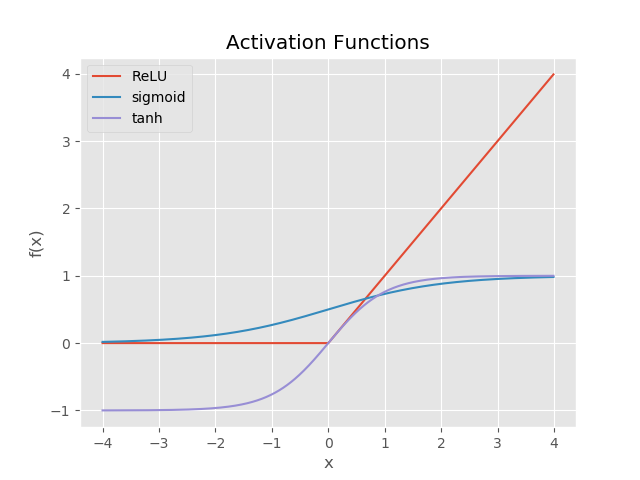
\includegraphics[width=0.5\textwidth]{Assets/Chapter2_Theory/activation_function_overview.png}
    \caption{Three activation functions plotted from x = -4 to x = 4.}
\end{figure}
\textbf{Relu}


\textbf{Softmax}

\textbf{Tanh}

\textbf{Sigmoid}

\subsubsection{Propagation function}
% backpropagation
% more details about changing weights
% math formulas

\subsubsection{Loss functions}
% gradient descent
% math formulas
% illustrations

\subsubsection{The dropout layer}

% Simple explanation and illustration
% drop random weightchanges
% to prevent overfitting
% https://www.cs.toronto.edu/~hinton/absps/JMLRdropout.pdf
% 

\subsection{Types of artificial neural networks}

\subsubsection{Feedforward neural networks}
% 

\subsubsection{Convolutional neural networks}
% is feedforward with convolutional mathematical operations between some layers
% convolutional layers: conv_1d, 2d, explain kernels
% explaing pooling layers
% image recognition
% pros cons
% 

\subsubsection{Recurrent neural networks}
% sequences
% time dimension
% pros cons

\subsubsection{Long short-term memory networks} % should this be a subsection of recurrent nets?
% also RNN
% goes further back in timesteps
% pros cons
